\providecommand{\gcph}[1]{\par\noindent\fbox{\parbox{0.6\textwidth}{\centering\small\color{red}[GC SCREEN PLACEHOLDER] #1}}\par\smallskip}
%% ============================================================ 71  ASRJC 2025 Prelim P1 Q8
\defQ{71}{}{%
\begin{qparts}
\pt{(a)}
\begin{qparts}
\pt{(i)} The ninth, fifth and second terms of an arithmetic progression are successive terms of a geometric progression with first term $a$ and common ratio $r$, where $r\neq1$ and $a>0$. Find the value of $r$ and deduce that the geometric series is convergent. \mk{3}
\pt{(ii)} Using the value of $r$ found in (i), find the least value of $n$ such that the sum of all the terms after the $n$th term of the geometric progression is less than 1\% of its sum of the first $n$ terms. \mk{3}
\end{qparts}
\pt{(b)} The sum, $S_n$, of the first $n$ terms of another sequence is given by $S_n=n\ln2^{q(n+1)}$, where $q$ is a constant. Prove that the sequence follows an arithmetic progression. \mk{4}
\end{qparts}
\src{ASRJC 2025 Prelim P1 Q8}}
\defS{71}{%
\begin{gtpart}{(a)(i)}{3}Let the first term and common difference of the arithmetic progression be $b$ and $d$ respectively.\par
Since $b+8d$, $b+4d$ and $b+d$ are successive terms of a GP, then $\dfrac{b+4d}{b+8d}=\dfrac{b+d}{b+4d}$ (common ratio).
\begin{topalign}
(b+4d)^{2}&=(b+8d)(b+d)\\8bd+16d^{2}&=9bd+8d^{2}\\d(8d-b)&=0\\b&=8d\quad(d\neq0)\\\Rightarrow r&=\frac{8d+4d}{8d+8d}=\frac34
\end{topalign}
Since $|r|=\left|\dfrac34\right|<1$, the series is convergent.\end{gtpart}
\begin{gtpart}{(a)(ii)}{3}$S_\infty-S_n<0.01S_n\ \Rightarrow\ S_\infty<1.01S_n$
\begin{topalign}
\frac{a}{1-\frac34}&<1.01\left[\frac{a\left(1-\left(\frac34\right)^{n}\right)}{1-\frac34}\right]\\1&<1.01\left(1-\left(\frac34\right)^{n}\right)\\\left(\frac34\right)^{n}&<0.009901\\n\ln\left(\frac34\right)&<\ln(0.009901)\\n&>\frac{\ln(0.009901)}{\ln\left(\frac34\right)}=16.042
\end{topalign}
Hence least $n$ is 17.\end{gtpart}
\begin{gtpart}{(b)}{4}\begin{topalign}
T_n=S_n-S_{n-1}&=n\ln2^{q(n+1)}-(n-1)\ln2^{q(n)}\\&=n(n+1)q\ln2-(n-1)(nq)\ln2\\&=nq\ln2+nq\ln2\\&=2nq\ln2\\&\fhl{\color{gray}\small Check: $T_1=S_1=2q\ln2$ (as $T_n=S_n-S_{n-1}$ only holds for $n\geq2$)}\\T_n-T_{n-1}&=2nq\ln2-2(n-1)q\ln2\\&=2q\ln2\quad(\text{constant}\ \because q\text{ is a constant})
\end{topalign}
$\therefore$ the sequence is an arithmetic progression (Proved).\end{gtpart}}
%% ============================================================ 72  TMJC 2025 Prelim P1 Q4
\defQ{72}{}{%
An arithmetic series has first term $a$ and common difference $d$, where $a$ and $d$ are non-zero real constants. A convergent geometric series has first term $b$ and common ratio $r$, where $b>0$ and $r$ is a non-zero real constant. The sum of the first $n$ terms of the geometric series is denoted by $S$.\par
It is given that the 7th, 10th and 11th terms of the arithmetic series are equal to the 3rd, 6th and 10th terms of the geometric series respectively.
\begin{qparts}
\pt{(a)} Show that $r$ satisfies the equation $3r^{7}-4r^{3}+1=0$. Solve this equation, giving your answer correct to 4 decimal places. \mk{4}
\pt{(b)} A new series is formed by taking the even numbered terms of the geometric series. Find the smallest value of $n$ for which $S$ differs from the sum to infinity of the new series by at least $1.78b$. \mk{4}
\end{qparts}
\src{TMJC 2025 Prelim P1 Q4}}
\defS{72}{%
\begin{gtpart}{(a)}{4}\begin{topalign}
a+6d&=br^{2}\quad--\ (1)\\a+9d&=br^{5}\quad--\ (2)\\a+10d&=br^{9}\quad--\ (3)\\(2)-(1):\ 3d&=br^{2}\left(r^{3}-1\right)\quad--\ (4)\\(3)-(2):\ d&=br^{5}\left(r^{4}-1\right)\quad--\ (5)
\end{topalign}
Substitute (5) into (4),
\begin{topalign}
3br^{5}\left(r^{4}-1\right)&=br^{2}\left(r^{3}-1\right)\\3r^{3}\left(r^{4}-1\right)&=\left(r^{3}-1\right)\quad(\text{since }b,r\neq0)\\3r^{7}-4r^{3}+1&=0\quad(\text{shown})
\end{topalign}
By GC, since the series is convergent, $|r|<1$,\par $r=0.6639$ (4 d.p.)
\par\smallskip{\centering\fhl{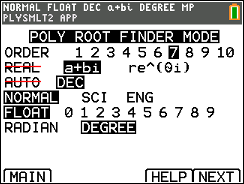
\includegraphics[width=0.31\linewidth]{gc/72_gc1.png}}\hfill\fhl{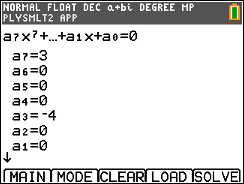
\includegraphics[width=0.31\linewidth]{gc/72_gc2.png}}\hfill\fhl{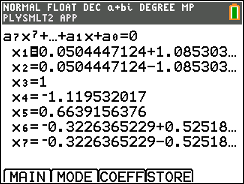
\includegraphics[width=0.31\linewidth]{gc/72_gc3.png}}\par}\end{gtpart}
\begin{gtpart}{(b)}{4}New Series: $br,br^{3},br^{5},\dots$
\begin{topalign}
\left|\frac{br}{1-r^{2}}-S\right|&\geqslant1.78b\\\left|\frac{br}{1-r^{2}}-\frac{b}{1-r}\left(1-r^{n}\right)\right|&\geqslant1.78b\\\left|\frac{0.6639b}{1-0.6639^{2}}-\frac{b}{1-0.6639}\left(1-0.6639^{n}\right)\right|&\geqslant1.78b\\\left|\frac{0.6639}{1-0.6639^{2}}-\frac{1}{1-0.6639}\left(1-0.6639^{n}\right)\right|&\geqslant1.78\quad(\because b>0)
\end{topalign}
Using GC,
\begin{topalign}
&\text{When }n=14,\ \left|\frac{0.6639}{1-0.6639^{2}}-\frac{1}{1-0.6639}\left(1-0.6639^{n}\right)\right|=1.7785<1.78\\&\text{When }n=15,\ \left|\frac{0.6639}{1-0.6639^{2}}-\frac{1}{1-0.6639}\left(1-0.6639^{n}\right)\right|=1.7818\geqslant1.78
\end{topalign}
Therefore, least $n=15$.\end{gtpart}}
%% ============================================================ 73  SAJC 2025 Prelim P1 Q5
\defQ{73}{}{%
An arithmetic progression has first term $a$ and common difference $d$, where $a$ and $d$ are non-zero. The 3rd, 9th and 11th terms of the arithmetic progression are three distinct consecutive terms of a geometric progression.
\begin{qparts}
\pt{(a)} Find $d$ in terms of $a$. \mk{3}
\pt{(b)} Let the sum of the first $n$ terms of the arithmetic progression be $S_n$ where $S_1=143$. Find the largest possible value of $S_n$. \mk{3}
\end{qparts}
The first term of the geometric progression is $b$, where $b$ is positive.
\begin{qparts}
\pt{(c)} Determine whether the geometric series is convergent. \mk{2}
\pt{(d)} Show that the sum of all terms after the $n$th term of the geometric progression is at most $\frac12b$, where $n$ is a positive integer. \mk{2}
\end{qparts}
\src{SAJC 2025 Prelim P1 Q5}}
\defS{73}{%
\begin{gtpart}{(a)}{3}\begin{topalign}
\frac{a+8d}{a+2d}&=\frac{a+10d}{a+8d}\\(a+8d)^{2}&=(a+2d)(a+10d)\\a^{2}+16ad+64d^{2}&=a^{2}+12ad+20d^{2}\\4ad+44d^{2}&=0\\4d(a+11d)&=0
\end{topalign}
$d=0$ (reject since terms of AP, GP are distinct)\quad or\quad $a+11d=0$\par
\hspace*{0.5\linewidth}$d=-\dfrac{1}{11}a$\end{gtpart}
\begin{gtpart}{(b)}{3}\begin{topalign}
S_1=a&=143\\d&=-\frac{1}{11}(143)=-13\\S_n&=\frac{n}{2}\left[2a+(n-1)d\right]\\&=\frac{n}{2}\left[286-13(n-1)\right]
\end{topalign}
From GC, largest $S_n=858$
\par\smallskip{\centering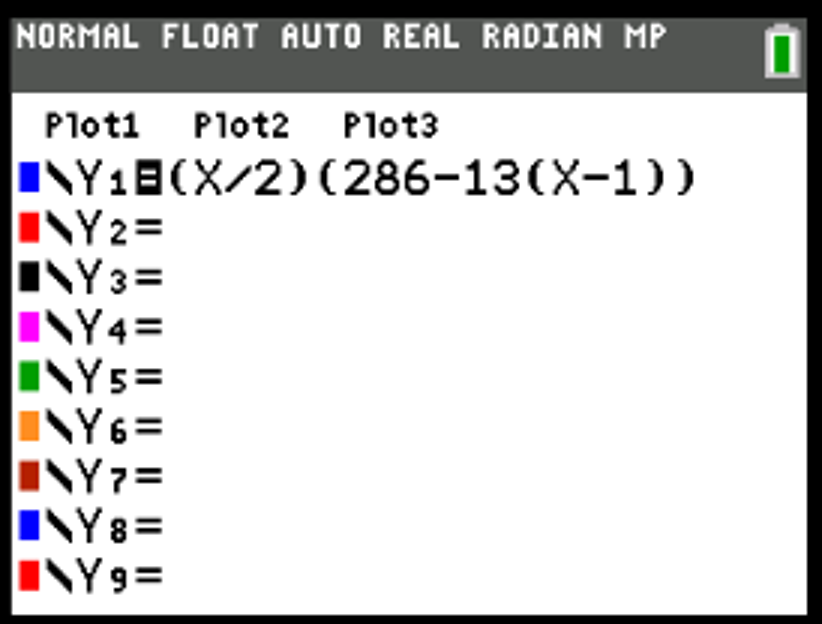
\includegraphics[width=0.48\linewidth]{gc/73_gc1.png}\hfill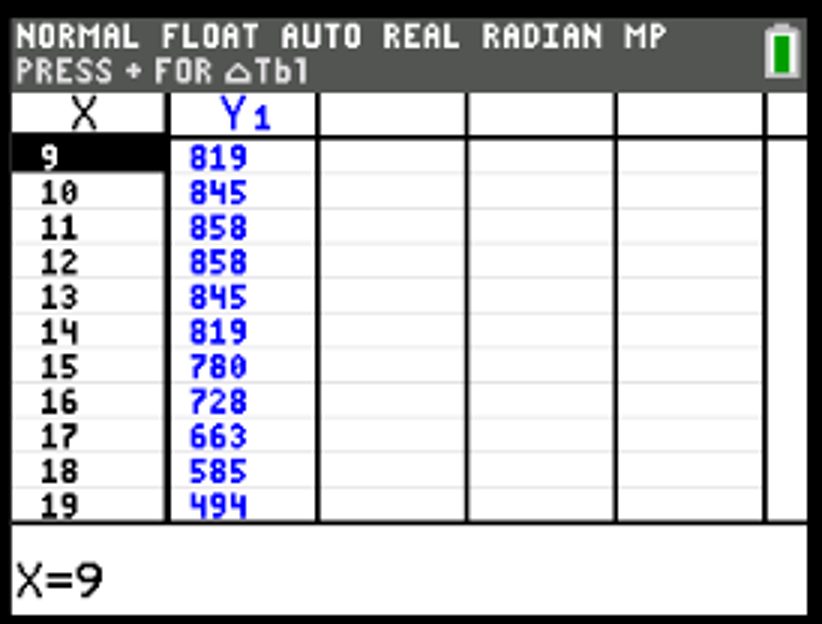
\includegraphics[width=0.48\linewidth]{gc/73_gc2.png}\par}
\end{gtpart}
\begin{gtpart}{(c)}{2}\begin{topalign}
r=\frac{a+8d}{a+2d}=\frac{-11d+8d}{-11d+2d}=\frac{-3d}{-9d}=\frac13
\end{topalign}
Since $|r|=\dfrac13<1$, the geometric series is convergent.\end{gtpart}
\begin{gtpart}{(d)}{2}Let $u_n$ be the $n$th term of the geometric progression.
\begin{topalign}
&u_{n+1}+u_{n+2}+\dots\\&=S_\infty-S_n\\&=\frac{b}{1-r}-\frac{b\left(1-r^{n}\right)}{1-r}\\&=\frac{br^{n}}{1-r}\\&=\frac{b\left(\frac13\right)^{n}}{1-\frac13}\\&=\frac32\left(\frac13\right)^{n}b\\&=\frac{b}{2}\left(\frac13\right)^{n-1}\leqslant\frac12b\quad\text{since }\left(\frac13\right)^{n-1}\leqslant1
\end{topalign}
Alternative:
\begin{topalign}
&u_{n+1}+u_{n+2}+u_{n+3}+\dots\\&=b\left(\frac13\right)^{n}+b\left(\frac13\right)^{n+1}+b\left(\frac13\right)^{n+2}+\dots\\&=\frac{b\left(\frac13\right)^{n}}{1-\frac13}\\&=\frac32b\left(\frac13\right)^{n}\\&=\frac{b}{2}\left(\frac13\right)^{n-1}\leqslant\frac{b}{2}\quad\text{since }\left(\frac13\right)^{n-1}\leqslant1
\end{topalign}\end{gtpart}}
%% ============================================================ 74  TJC 2025 Prelim P1 Q7
\defQ{74}{}{%
Mabel and Janice decided to start a 5-year savings plan beginning in January 2026.\par
Mabel saves using a piggy bank. At the start of January 2026, she deposits \$101. Each subsequent month, she increases her deposit by \$1---so she deposits \$101 in January, \$102 in February, \$103 in March, and so on, until \$112 in December. At the start of each new year, she resets her monthly deposit to \$101 in January and repeats the same pattern through December. She continues this routine from 2026 to 2030, inclusive.\par
Janice, on the other hand, deposits \$100 at the start of every month into a bank account that earns 0.3\% interest per month, with interest calculated and added into the account at the end of each month.
\begin{qparts}
\pt{(a)} Show that Janice will have more money in her savings account than Mabel has in her piggy bank at the end of December 2030. \mk{5}
\pt{(b)} Find the month and year when Janice's savings first exceed Mabel's savings. \mk{4}
\end{qparts}
\src{TJC 2025 Prelim P1 Q7}}
\defS{74}{%
\begin{gtpart}{(a)}{5}For Mabel:\par
Amount of money Mabel saves in a year
\begin{topalign}
&=\$(101+102+\dots+112)\\&=\$\frac{12}{2}(101+112)=\$1278
\end{topalign}
Amount of money Mabel saves in 5 year $=\$1278\times5=\$6390$\par\medskip
For Janice:\par\smallskip
{\small\renewcommand{\arraystretch}{1.3}\begin{tabular}{|l|l|l|}\hline
$n$th mth&Amount at start of month (\$)&Amount at end of month (\$)\\\hline
1 Jan26&$100$&$100(1.003)$\\\hline
2&$\begin{aligned}[t]&100+100(1.003)\\&=100(1+1.003)\end{aligned}$&$\begin{aligned}[t]&100(1+1.003)(1.003)\\&=100\left(1.003+1.003^{2}\right)\end{aligned}$\\\hline
$\vdots$&&$\vdots$\\\hline
$n$&&$\begin{aligned}[t]&100\left(1.003+1.003^{2}+\dots+1.003^{n}\right)\\&=\frac{100(1.003)\left(1.003^{n}-1\right)}{1.003-1}\end{aligned}$\\\hline
\end{tabular}}\par\medskip
At Dec 2030, $n=60$.\par
Therefore, Amount Janice saves in 5 years
\begin{topalign}
=\frac{100(1.003)\left(1.003^{60}-1\right)}{1.003-1}=\$6582.85\ \text{(2 d.p.) [A1]}
\end{topalign}
$\therefore$ Janice will have more money in her savings account than Mabel has in her piggy bank.\end{gtpart}
\begin{gtpart}{(b)}{4}At end of 4\textsuperscript{th} year,\par
Mabel will have \$1278 x 4 $=\$5112$\par
Janice will have $\dfrac{100(1.003)\left(1.003^{48}-1\right)}{1.003-1}=\$5169.97>\$5112$\par\smallskip
At end of 3\textsuperscript{rd} year,\par
Mabel will have \$1278 x 3 $=\$3834$\par
Janice will have $\dfrac{100(1.003)\left(1.003^{36}-1\right)}{1.003-1}=\$3806.97<\$3834$\par\smallskip
Therefore, the year when Janice's saving is more than Mabel's saving happen in 4\textsuperscript{th} year (i.e. 2029). Let it be the $k$\textsuperscript{th} month.\par
Then set Janice's saving $>$ Mabel's saving
\begin{topalign}
&\Rightarrow\frac{100(1.003)\left(1.003^{36+k}-1\right)}{1.003-1}>3834+\frac{k}{2}\left[2(100)+(k-1)(1)\right]\\&\Rightarrow\left(\frac{100003}{3}\right)\left(1.003^{36+k}-1\right)-3834-\frac{k}{2}\left[199+k\right]>0
\end{topalign}
Using GC, we have $k\geqslant4$. Therefore, the month and year is Apr 2029.\end{gtpart}}
%% ============================================================ 75  ACJC 2025 Prelim P1 Q12
\defQ{75}{}{%
Sarah, a Singaporean Citizen, started a 4-year undergraduate Computing course at the National University of Singapore (NUS) in August 2021. The annual tuition fee, after the MOE Tuition Grant, is \$8,250. Sarah took a Tuition Fee Loan (TFL) covering 90\% of her tuition fees. This loan is interest-free during her course of study.\par
Sarah decided to set aside \$$x$ per month from August 2021. This amount is increased by \$2 each subsequent month. (Sarah set aside \$$x$ in August 2021, \$$(x+2)$ in September 2021, \dots.) With the amount set aside, she repaid one-fifth of her total TFL at the end of July 2025.
\begin{qparts}
\pt{(a)} Find the value of $x$. \mk{3}
\end{qparts}
Upon Sarah's graduation, the TFL's interest rate becomes effective at a fixed rate of 0.4\% per month, calculated on the outstanding balance at the end of the month. The interest is first charged on 31st August 2025.\par
Sarah plans to make monthly repayments of \$$y$ to the bank on the 1st of every month, starting from 1st September 2025.
\begin{qparts}
\pt{(b)} Find the amount of outstanding loan after Sarah's first monthly repayment. \mk{1}
\pt{(c)} Show that the amount of outstanding loan after Sarah's $n$th monthly repayment is
\[23760(1.004)^{n}-250y\left(1.004^{n}-1\right).\] \mk{3}
\pt{(d)} Sarah wants to pay off her remaining loan by the end of 3 years. Find the value of $y$. \mk{2}
\end{qparts}
Sarah decided on a different repayment strategy. For the first 24 months, she repays \$500 per month. After these 24 months, she doubles her monthly repayment to \$1000.
\begin{qparts}
\pt{(e)} Determine the month and year Sarah will clear her loan and calculate the amount of her final repayment. \mk{4}
\end{qparts}
\src{ACJC 2025 Prelim P1 Q12}}
\defS{75}{%
\begin{gtpart}{(a)}{3}Amount Sarah plans to repay (before graduation):\par
$\dfrac15\times\dfrac{90}{100}\times8250\times4=\$5940$\par\smallskip
Number of repayments made from August 2021 to July 2025 is 48 (i.e. $n=48$).\par
The repayments follow an arithmetic progression (AP) with first term $a=x$ and common difference $d=2$.\par\smallskip
The sum of an arithmetic progression is
\begin{topalign}
S_n&=\frac{n}{2}\left[2a+(n-1)d\right]\\5940&=\frac{48}{2}\left[2x+(48-1)2\right]\\x&=76.75
\end{topalign}\end{gtpart}
\begin{gtpart}{(b)}{1}Amount of outstanding loan after Sarah's graduation:\par
$\dfrac45\times\dfrac{90}{100}\times8250\times4=\$23760$\par\smallskip
On 31\textsuperscript{st} August 2025, apply interest of 0.4\% to outstanding loan to get $\$\left(23760(1.004)\right)$.\par
On 1\textsuperscript{st} September 2025, make 1\textsuperscript{st} repayment of \$$y$ to the bank.\par\smallskip
$\therefore$ Outstanding loan after 1\textsuperscript{st} repayment\par
$=\$\left(23760(1.004)-y\right)$ or $\$(23855.04-y)$\end{gtpart}
\begin{gtpart}{(c)}{3}On 30\textsuperscript{th} September 2025, apply interest of 0.4\%.\par
On 1\textsuperscript{st} October 2025, make 2\textsuperscript{nd} repayment of \$$y$.\par
Outstanding loan after 2\textsuperscript{nd} repayment
\begin{topalign}
&=\left(23760(1.004)-y\right)1.004-y\\&=23760(1.004)^{2}-1.004y-y
\end{topalign}
Outstanding loan after 3\textsuperscript{rd} repayment (on 1\textsuperscript{st} Nov 2025)
\begin{topalign}
&=\left(23760(1.004)^{2}-1.004y-y\right)1.004-y\\&=23760(1.004)^{3}-1.004^{2}y-1.004y-y
\end{topalign}
Outstanding loan after $n$\textsuperscript{th} repayment
\begin{topalign}
&=23760(1.004)^{n}-1.004^{n-1}y-\dots-1.004^{2}y-1.004y-y\\&=23760(1.004)^{n}-y\left(1+1.004+1.004^{2}+\dots+1.004^{n-1}\right)\\&=23760(1.004)^{n}-y\left(\frac{1.004^{n}-1}{1.004-1}\right)\\&=23760(1.004)^{n}-250y\left(1.004^{n}-1\right)\ \text{(shown)}
\end{topalign}\end{gtpart}
\begin{gtpart}{(d)}{2}To repay remaining loan by the end of 3 years (i.e. 36 monthly repayments of \$$y$), let $n=36$.\par\smallskip
To fully repay the loan, we want outstanding loan amount after 36 repayments to be zero (or less).
\begin{topalign}
23760(1.004)^{36}-250y\left(1.004^{36}-1\right)&\leqslant0\\y&\geqslant709.9769\\\therefore\ y&=709.98\ \text{(nearest cent)}
\end{topalign}\end{gtpart}
\begin{gtpart}{(e)}{4}After 24 monthly repayments of \$500 (i.e. $n=24$, $y=500$), outstanding loan amount
\begin{topalign}
&=23760(1.004)^{24}-250(500)\left((1.004)^{24}-1\right)\\&=13580.49
\end{topalign}
Outstanding loan amount as of 1\textsuperscript{st} August 2027\par
$=13580.49$\par
In a similar method to \textbf{(c)}, the outstanding loan amount after $m$ monthly repayments of \$1000 (i.e. $y=1000$) is\par
$13580.49(1.004)^{m}-250(1000)\left((1.004)^{m}-1\right)$\par\smallskip
To fully repay the loan, we need
\begin{topalign}
13580.49(1.004)^{m}-250(1000)\left((1.004)^{m}-1\right)&\leqslant0\\m&\geqslant13.991185\\\text{Least }m&=14
\end{topalign}
Sarah would require another 14 monthly repayments to fully repay her loan, with her first repayment of \$1000 on 1\textsuperscript{st} September 2027.\par\smallskip
Hence, she would clear her loan on \underline{(1st) October 2028}.\par\smallskip
The outstanding loan amount after her 13\textsuperscript{th} monthly repayment of \$1000 (on 1\textsuperscript{st} Sep 2028) is
\begin{topalign}
&13580.49(1.004)^{13}-250(1000)\left((1.004)^{13}-1\right)\\&=987.2529
\end{topalign}
Interest is applied on 30\textsuperscript{th} Sep 2028. Hence her final repayment amount is\par
$987.2529\times1.004=\underline{\$991.20}$ (nearest cent)\par\smallskip
(Alternatively, outstanding loan amount after 14\textsuperscript{th} monthly repayment is
\begin{topalign}
&13580.49(1.004)^{14}-250(1000)\left((1.004)^{14}-1\right)\\&=-8.7981
\end{topalign}
Hence the final repayment is $1000-8.7981=\$991.20$ (nearest cent).\end{gtpart}}
%% ============================================================ 76  RVHS 2025 Prelim P2 Q4
\defQ{76}{}{%
The dosage of medicine given to a patient needs to be carefully managed in order to achieve the desired result.
\begin{qparts}
\pt{(a)} To give the patient time to adapt to a particular medicine, the dosage is slowly increased over time. The patient is initially given a dosage of 0.75 units. The dosage is increased by 0.5 units each day until a total of at least 10 units of medicine has been taken. Find the least number of days it takes to achieve this, and the dosage on that day. \mk{4}
\pt{(b)} The doctor prescribed a new medication to another patient. After $n$ days, the total dosage of the new medicine administered to the patient is given by
\[\frac{3}{20}\left(\frac{5^{n}-4^{n}}{5^{n-1}}\right)\ \text{units.}\]
\begin{qparts}
\pt{(i)} Show that the increase in dosage of the new medicine administered per day follows a geometric progression. \mk{3}
\pt{(ii)} Find the total dosage of the new medicine administered to the patient after a long period of treatment. \mk{2}
\end{qparts}
\pt{(c)} Doctors can manage the medication so that the daily dosage of medicine increases as an arithmetic progression. Explain in context why the arithmetic progression is not a preferred model for the dosage of medication. \mk{1}
\end{qparts}
\src{RVHS 2025 Prelim P2 Q4}}
\defS{76}{%
\begin{gtpart}{(a)}{4}Let $u_n$ be the dose on the $n^{th}$ day.
\begin{topalign}
u_n&=0.75+0.5(n-1)\\S_n&=\frac{n}{2}\left(2(0.75)+(n-1)(0.5)\right)\\10&\leqslant\frac{n}{2}\left(1+\frac{n}{2}\right)\qquad\text{-----}(*)\\\frac14n^{2}+\frac12n&\geqslant10\\n^{2}+2n&\geqslant40\\(n+1)^{2}&\geqslant41\\n\geqslant-1+\sqrt{41}\ &\text{or}\ n\leqslant-1-\sqrt{41}\\&\text{(rej as no. of days cannot be -ve)}\\n&\geqslant5.40312
\end{topalign}
Therefore, it takes 6 days.\par\smallskip
Alternatively,\par
When $n=5$, $\frac14n^{2}+\frac12n=8.75<10$\par
When $n=6$, $\frac14n^{2}+\frac12n=12\geqslant10$\par
Therefore, it takes 6 days.\par\smallskip
$u_6=0.75+0.5(5)=3.25$\par
The dose on the 6\textsuperscript{th} day is 3.25 units.\end{gtpart}
\begin{gtpart}{(b)(i)}{3}Increase on $n^{th}$ day
\begin{topalign}
&=S_n-S_{n-1}\\&=\frac{3}{20}\left(\frac{5^{n}-4^{n}}{5^{n-1}}\right)-\frac{3}{20}\left(\frac{5^{n-1}-4^{n-1}}{5^{n-2}}\right)\\&=\frac{3}{20}\left(\frac{5^{n}-4^{n}}{5^{n-1}}-\frac{5^{n-1}-4^{n-1}}{5^{n-2}}\right)\\&=\frac{3}{20}\left(\frac{1}{5^{n-2}}\right)\left(5^{n-1}-\frac45\left(4^{n-1}\right)-5^{n-1}+4^{n-1}\right)\\&=\frac{3}{20}\left(\frac{1}{5^{n-2}}\right)\left(\frac15\right)\left(4^{n-1}\right)\\&=\frac{3}{20}\left(\frac45\right)^{n-1}
\end{topalign}
which is of the form $ar^{n-1}$, where $a=\dfrac{3}{20}$ and $r=\dfrac45$ which is a GP.\par\smallskip
\textbf{\underline{Alternative:}}\par
Consider $\dfrac{u_{n+1}}{u_n}=\dfrac{\frac{3}{20}\left(\frac45\right)^{n+1-1}}{\frac{3}{20}\left(\frac45\right)^{n-1}}=\dfrac45$ which is a constant\par\smallskip
Since consecutive terms have a common ratio $r=\dfrac45$, the increase in dosage follows a GP.\end{gtpart}
\begin{gtpart}{(b)(ii)}{2}\textbf{\underline{Method 1}}\par
Long term dosage
\begin{topalign}
&=\lim_{n\to\infty}\frac{3}{20}\left(\frac{5^{n}-4^{n}}{5^{n-1}}\right)\\&=\frac{3/20}{1-4/5}\\&=\frac34
\end{topalign}
In the long term, the total dosage approaches 0.75 units.\par\smallskip
\textbf{Note:}\par
After $n$ days, the total dosage of the medicine is given by $\dfrac{3}{20}\left(\dfrac{5^{n}-4^{n}}{5^{n-1}}\right)$.\par
Let $S_n$ denote the total dosage of the new medicine after $n$ days.\par
Then $S_n=\dfrac{3}{20}\left(\dfrac{5^{n}-4^{n}}{5^{n-1}}\right)$.\par
Let $v_n$ the change in dosage on $n$th day found in part (b)(i) where $v_n=S_n-S_{n-1}$\par
Since $v_n$ is a geometric progression, we can use $S_\infty=\dfrac{a}{1-r}$, the sum to infinity formula to find the long term total dosage.\par\smallskip
\textbf{\underline{Method 2}}
\begin{topalign}
&\frac{3}{20}\left(\frac{5^{n}-4^{n}}{5^{n-1}}\right)\\&=\frac{3}{20}(5)\left(\frac{5^{n}-4^{n}}{5^{n}}\right)\\&=\frac{3}{20}(5)\left(1-\left(\frac45\right)^{n}\right)
\end{topalign}
As $n\to\infty$, $\left(\dfrac45\right)^{n}\to0$\par
Total dosage in the long term
\begin{topalign}
&=\frac{3}{20}(5)(1-0)\\&=\frac34
\end{topalign}\end{gtpart}
\begin{gtpart}{(c)}{1}If the dosage increases as an AP, then it will continue to \textbf{\underline{increase to}} (positive) \textbf{\underline{infinity}}.\end{gtpart}}
